\begin{figure}[H]
    \centering
    \vspace{-2em}
    \textbf{(a)} Comparison with SOTA offline and optimization-based methods on Oxford-Spires \\[2pt]
    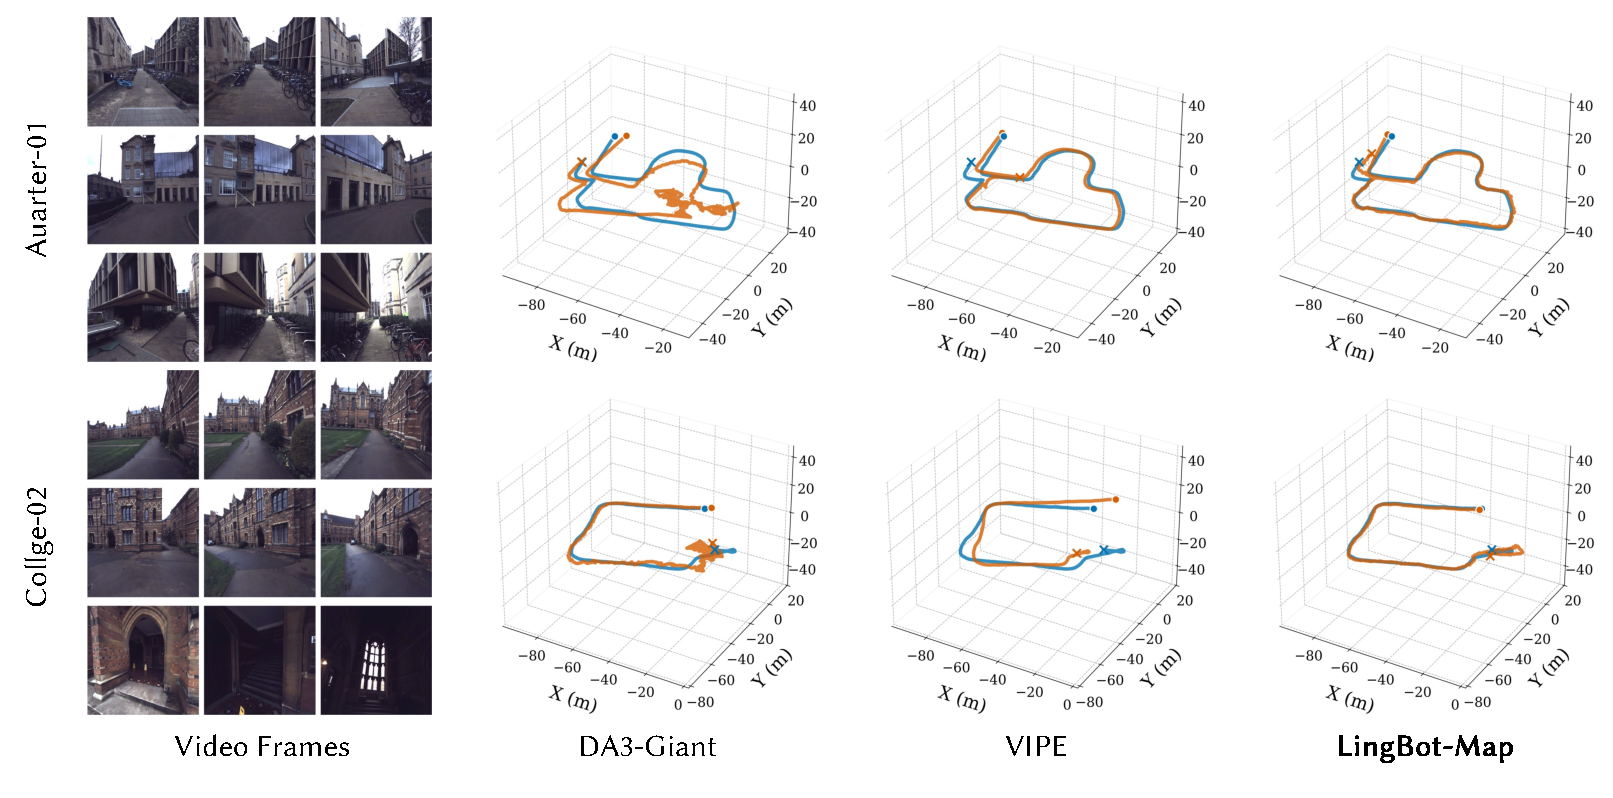
\includegraphics[width=0.9\textwidth]{figures/traj_comparison1.pdf}

    \vspace{3pt}

    \textbf{(b)} Comparison with SOTA streaming methods across diverse scenes \\[2pt]
    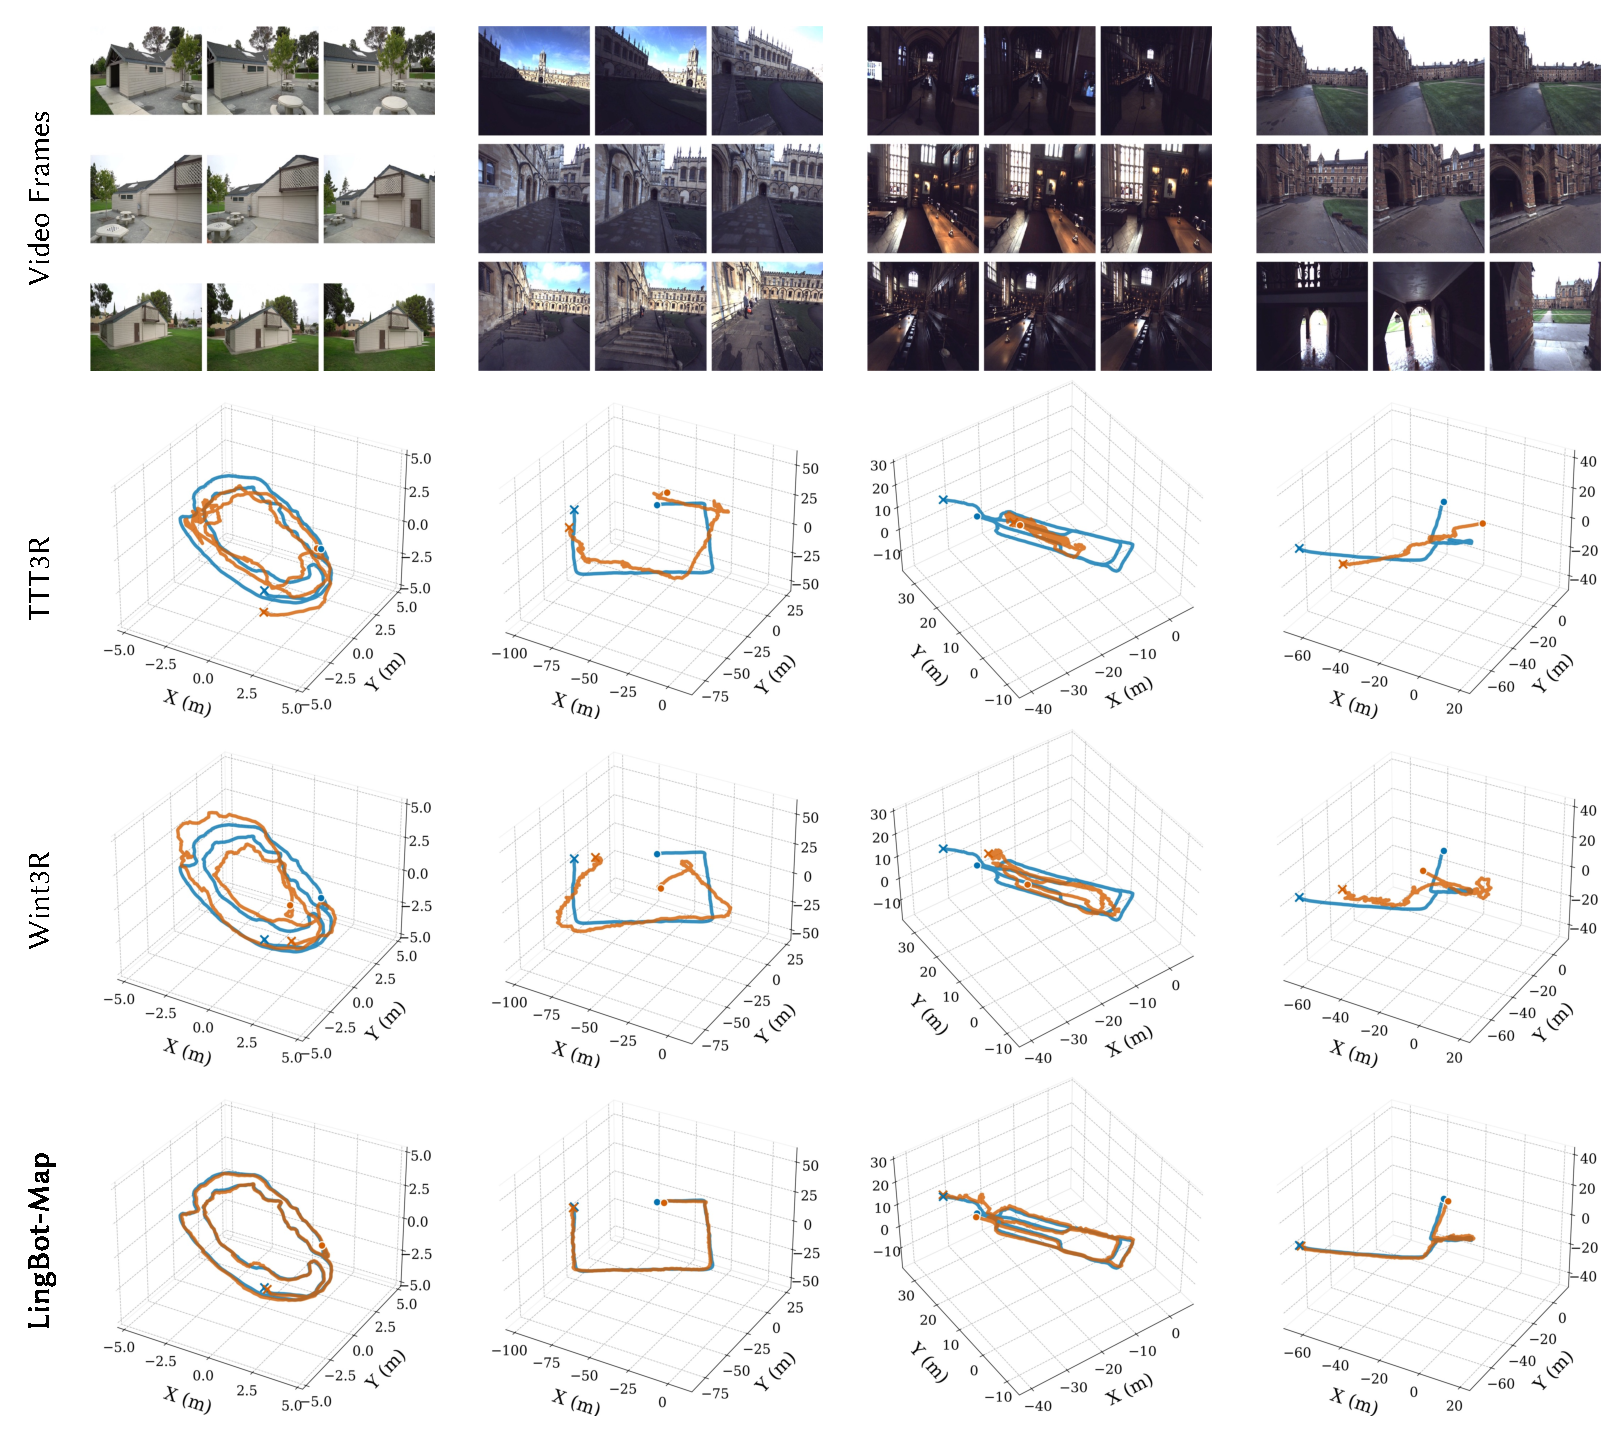
\includegraphics[width=0.9\textwidth]{figures/traj_comparison2.pdf}

    \definecolor{gtcolor}{RGB}{31, 119, 180}
    \definecolor{predcolor}{RGB}{255, 127, 14}

    \caption{\textbf{Trajectory comparison.}
    (a)~On Oxford-Spires, LingBot-Map even outperforms bidirectional (DA3-Giant), and optimization-based (ViPE) methods, accurately preserving trajectories during complex outdoor-to-indoor transitions and dark staircases.
    (b)~Across Tanks and Temples and additional Oxford-Spires scenes, our method consistently produces accurate trajectories while competing streaming methods suffer from severe drift.
    \textcolor{gtcolor}{Ground truth} in blue, \textcolor{predcolor}{predicted} in orange; start~{\textbullet}, end~\textbf{\texttimes}.}
    \label{fig:traj_results}
    \vspace{-8pt}
\end{figure}
